Инфологическая (концептуальная) модель предметной области представляет собой информационную модель наиболее высокого уровня абстракции и в сущности является как образом реальности, так и образом проектируемой базы данных для этой реальности. Она включает в себя описание информационных объектов или понятий предметной области и связей между ними. а также описание ограничений целостности, т.е. требований к допустимым значениям данных и к связям между ними.

Описание бизнесс-процессов в системе электронной регистрации пациентов представлено на диаграммах IDEF0, DFD IDEF3 (рисунки \ref{idef0_1:idef0_1}-\ref{}), представление модели <<Сущность-связь>> (ER-модель) --- на рисунке \ref{}.

\begin{figure}[h!]
\center{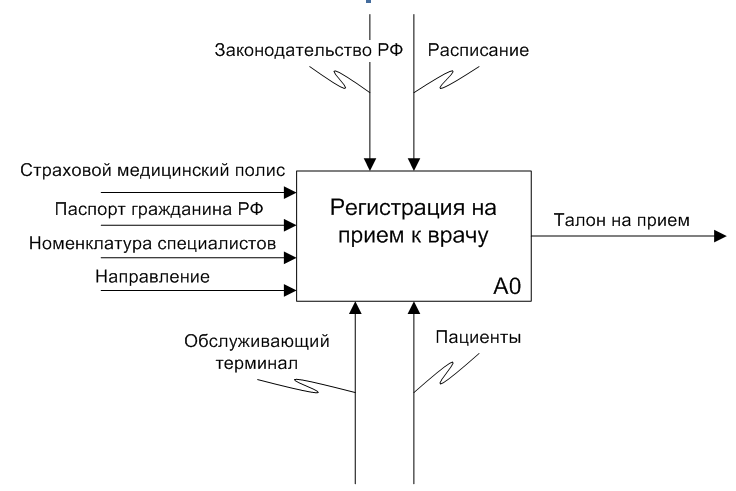
\includegraphics[width=0.9\linewidth]{idef0_1}}
\caption{<<Черный ящик>>}
\label{idef0_1:idef0_1}
\end{figure} 

\begin{figure}[h!]
\center{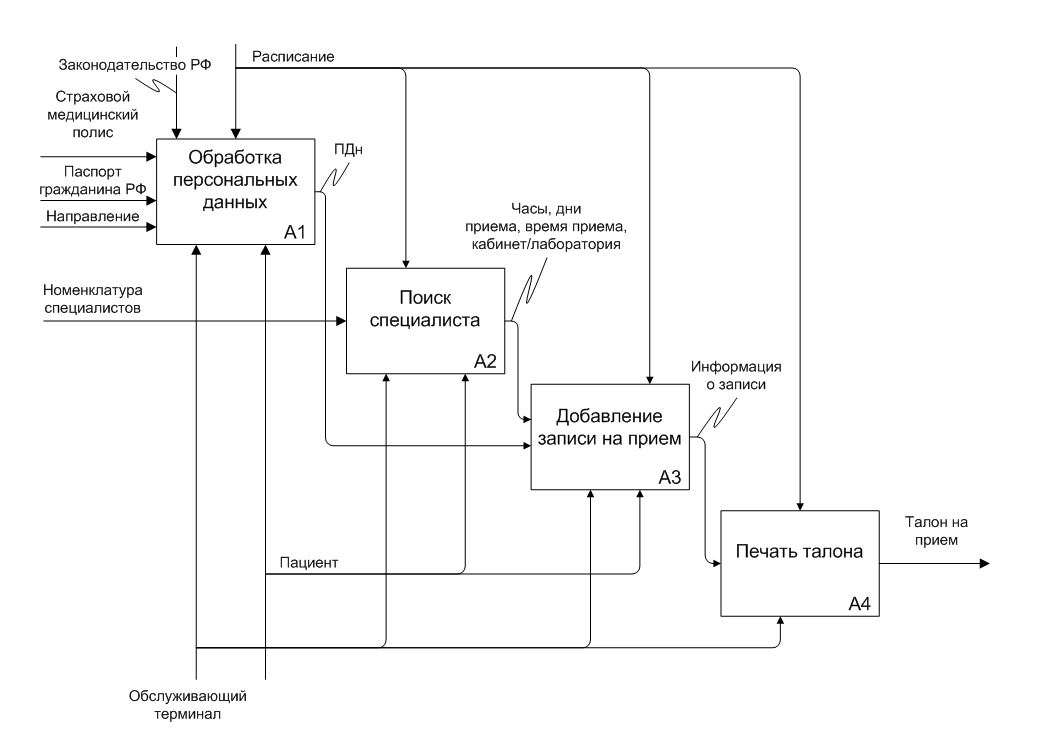
\includegraphics[width=0.9\linewidth]{idef0_2}}
\caption{Диаграмма IDEF0}
\label{idef0_2:idef0_2}
\end{figure} 

\begin{figure}[h!]
\center{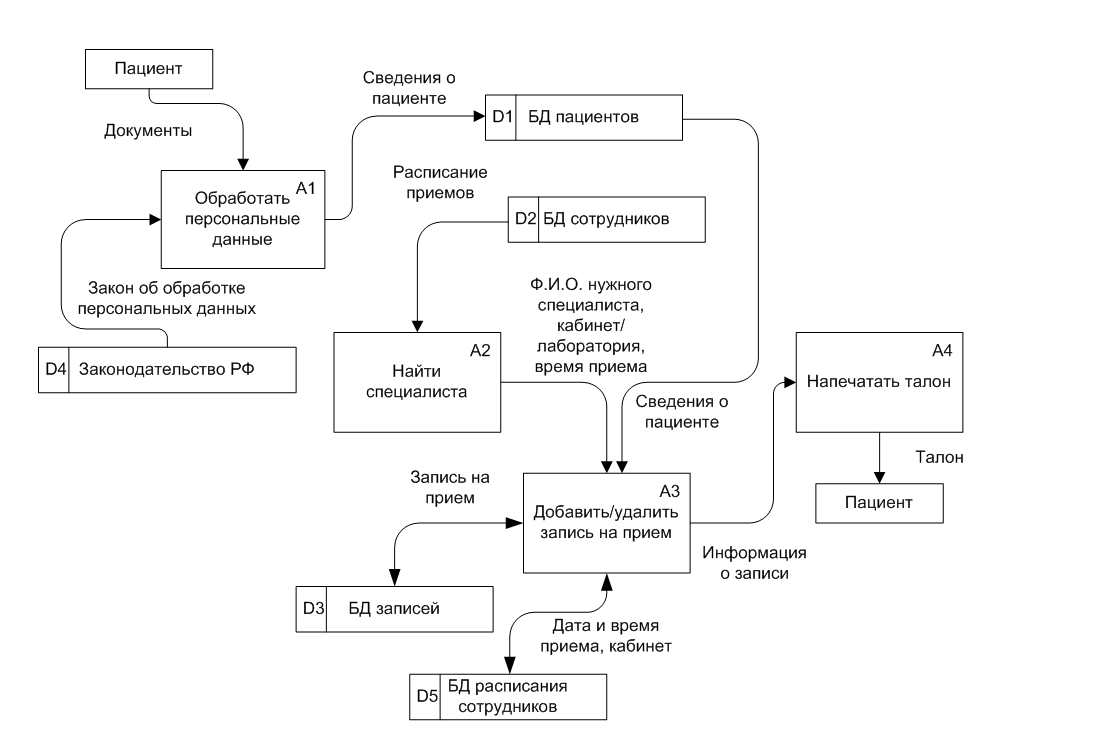
\includegraphics[width=0.9\linewidth]{dfd}}
\caption{DFD-диаграмма бизнес-процессов}
\label{dfd:dfd}
\end{figure} 

\begin{figure}[h!]
\center{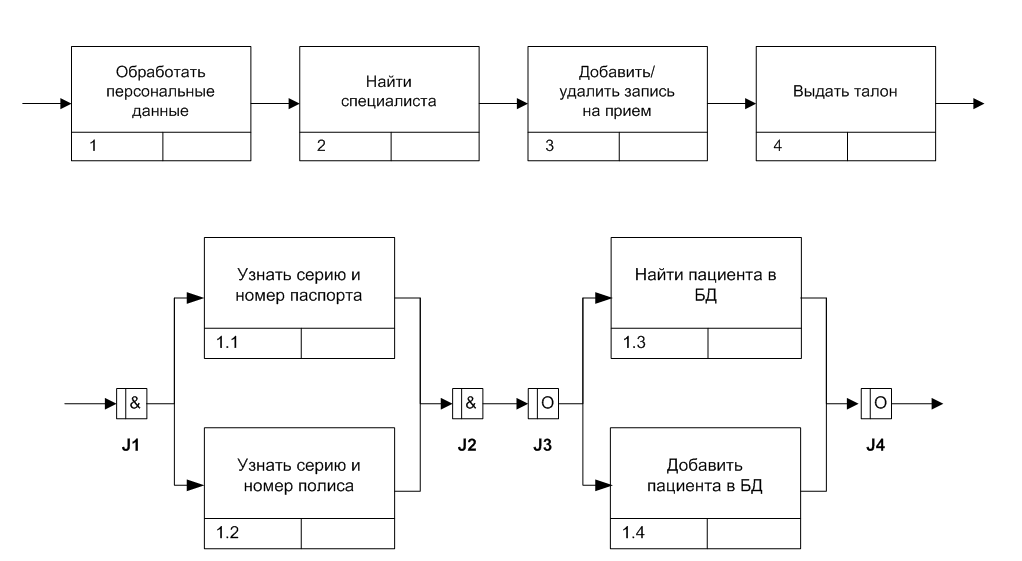
\includegraphics[width=0.9\linewidth]{idef3_1}}
\caption{Диаграмма IDEF3 (часть 1)}
\label{idef3_1:idef3_1}
\end{figure} 

\begin{figure}[h!]
\center{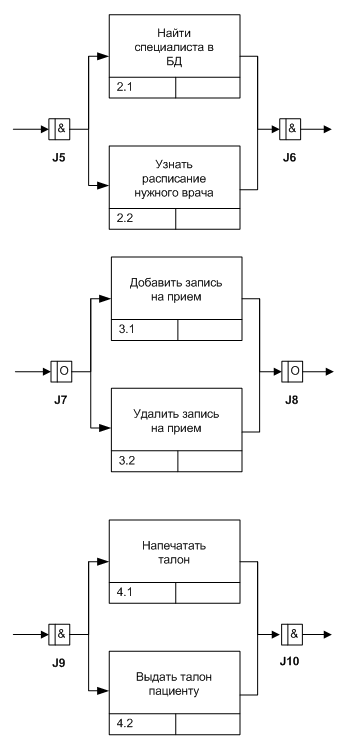
\includegraphics[width=0.9\linewidth]{idef3_2}}
\caption{Диаграмма IDEF3 (часть 2)}
\label{idef3_2:idef3_2}
\end{figure} 

\begin{figure}[h!]
\center{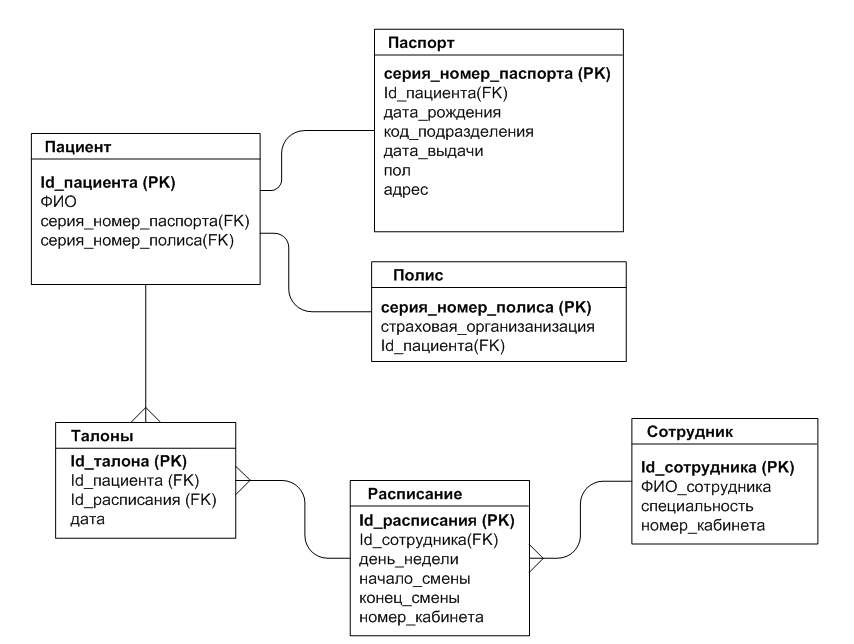
\includegraphics[width=0.9\linewidth]{idef1x}}
\caption{Диаграмма IDEF1X (модель <<Сущность-связь>>)}
\label{idef1x:idef1x}
\end{figure} 




